\section{Functionnal Architecture}

\subsection{Introduction}

\begin{figure}[!ht]
    \begin{center}
        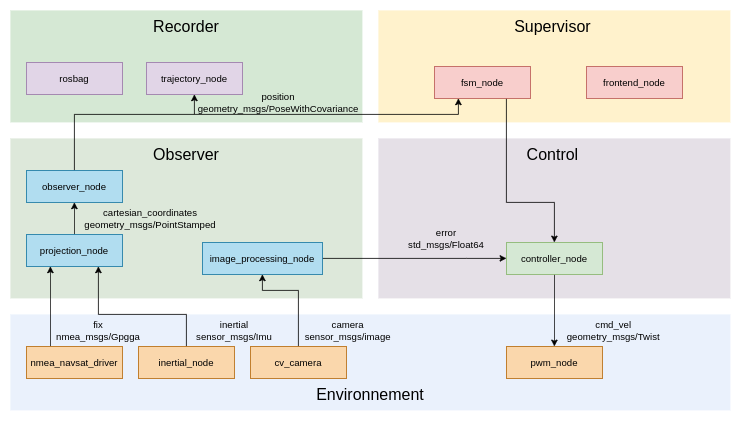
\includegraphics[scale=0.51]{Images/node_graph.png}
    \end{center}
    \caption{Functionnal Architecture of this project}
    \label{fig:requirement}
\end{figure}

The functionnal architecture constitutes the specifications of the project and allows us to have criteria
for the success of our project. \textbf{Figure}~\ref{fig:requirement} shows us the requirements
diagram that follows the \textit{SysML} standard for this system.

One can notice the presence of this architecture in two loops. We have a small loop formed
by the camera, image processing, controller and pwm nodes, and a much larger loop involving
the gps and the finite state machine. This relates well the will to want to achieve the
global mission by taking into account all the cases, to always have a command to give to
the car.

\newpage